\begin{figure}[ht]
\centering
% Thesis-wide categorical color palette
% Usage: % Thesis-wide categorical color palette
% Usage: % Thesis-wide categorical color palette
% Usage: \input{figures/palette} in any figure file
%
% Muted primary colors -- print-friendly, visually distinct.
% Inspired by Cooper Union's red/blue primaries, softened for
% academic figures. Use palA-palC for data series in scatter
% plots, line charts, bar charts, etc.

\definecolor{palA}{HTML}{1F77B4}   % Tableau blue
\definecolor{palB}{HTML}{D62728}   % Tableau red
\definecolor{palC}{HTML}{2CA02C}   % Tableau green
 in any figure file
%
% Muted primary colors -- print-friendly, visually distinct.
% Inspired by Cooper Union's red/blue primaries, softened for
% academic figures. Use palA-palC for data series in scatter
% plots, line charts, bar charts, etc.

\definecolor{palA}{HTML}{1F77B4}   % Tableau blue
\definecolor{palB}{HTML}{D62728}   % Tableau red
\definecolor{palC}{HTML}{2CA02C}   % Tableau green
 in any figure file
%
% Muted primary colors -- print-friendly, visually distinct.
% Inspired by Cooper Union's red/blue primaries, softened for
% academic figures. Use palA-palC for data series in scatter
% plots, line charts, bar charts, etc.

\definecolor{palA}{HTML}{1F77B4}   % Tableau blue
\definecolor{palB}{HTML}{D62728}   % Tableau red
\definecolor{palC}{HTML}{2CA02C}   % Tableau green


%% Panel (a): Filmstrip of 4 frames with ball at different positions
\begin{subfigure}{\textwidth}
\centering
\begin{tikzpicture}[
    lbl/.style={font=\footnotesize, text=black!55},
    dimlbl/.style={font=\scriptsize, text=black!45},
    tlbl/.style={font=\scriptsize, text=black!50},
]
\def\c{0.28}
\def\gs{5}  % 5x5 grid per frame

% Draw one frame: #1=x-offset, #2=ball-x (grid coords), #3=ball-y, #4=opacity
\newcommand{\drawframe}[4]{
    \foreach \x in {0,...,4} {
        \foreach \y in {0,...,4} {
            \fill[black!5, draw=black!12]
                ({#1 + \x*\c}, \y*\c) rectangle ++(\c, \c);
        }
    }
    % Ball
    \fill[palA!#4] ({#1 + (#2+0.5)*\c}, {(#3+0.5)*\c}) circle (0.11);
}

% Four frames with ball moving diagonally
\drawframe{0}{1}{1}{30}        % t-3: bottom-left
\drawframe{1.7}{2}{2}{45}      % t-2: center-left
\drawframe{3.4}{3}{3}{60}      % t-1: center-right
\drawframe{5.1}{4}{4}{100}     % t:   top-right

% Time labels below each frame
\node[tlbl] at ({2.5*\c}, {-0.2}) {$t{-}3$};
\node[tlbl] at ({1.7 + 2.5*\c}, {-0.2}) {$t{-}2$};
\node[tlbl] at ({3.4 + 2.5*\c}, {-0.2}) {$t{-}1$};
\node[tlbl] at ({5.1 + 2.5*\c}, {-0.2}) {$t$};

% Arrow to stacked output
\draw[->, thick, black!40]
    ({5.1 + 5*\c + 0.25}, {2.5*\c}) -- ++(0.5, 0);

% Output block
\node[draw=black!30, thick, rounded corners=2pt,
      minimum width=1.1cm, minimum height=1.3cm,
      fill=black!5, font=\scriptsize, align=center]
    at ({5.1 + 5*\c + 1.35}, {2.5*\c})
    {$84{\times}84$\\${\times}\,4$};

\end{tikzpicture}
\subcaption{Four consecutive frames capture the ball at different
  positions. Stacking them produces one multi-channel input.}
\label{fig:frame-stack-op}
\end{subfigure}

\vspace{1em}

%% Panel (b): Motion inference from the stacked frames
\begin{subfigure}{\textwidth}
\centering
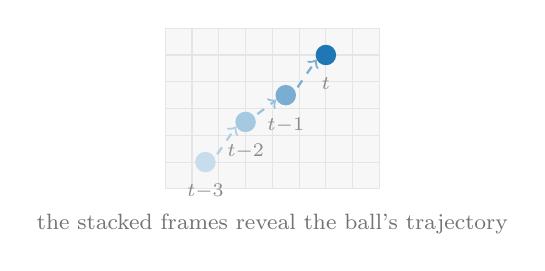
\begin{tikzpicture}[
    lbl/.style={font=\footnotesize, text=black!55},
    dimlbl/.style={font=\scriptsize, text=black!45},
]
\def\c{0.34}

% Game-like grid (8x6)
\foreach \x in {0,...,7} {
    \foreach \y in {0,...,5} {
        \fill[gray!6, draw=black!10]
            (\x*\c, \y*\c) rectangle ++(\c, \c);
    }
}

% Ball at four positions matching panel (a), increasing opacity
% t-3: bottom-left
\fill[palA!25] ({1.5*\c}, {1*\c}) circle (0.13);
\node[dimlbl, anchor=north] at ({1.5*\c}, {1*\c - 0.16})
    {$t{-}3$};

% t-2: left-center
\fill[palA!40] ({3*\c}, {2.5*\c}) circle (0.13);
\node[dimlbl, anchor=north] at ({3*\c}, {2.5*\c - 0.16})
    {$t{-}2$};

% t-1: right-center
\fill[palA!60] ({4.5*\c}, {3.5*\c}) circle (0.13);
\node[dimlbl, anchor=north] at ({4.5*\c}, {3.5*\c - 0.16})
    {$t{-}1$};

% t: upper-right
\fill[palA] ({6*\c}, {5*\c}) circle (0.13);
\node[dimlbl, anchor=north] at ({6*\c}, {5*\c - 0.16})
    {$t$};

% Dashed trajectory arrows
\draw[->, thick, dashed, palA!35]
    ({1.5*\c + 0.15}, {1*\c + 0.1})
    -- ({3*\c - 0.12}, {2.5*\c - 0.06});
\draw[->, thick, dashed, palA!45]
    ({3*\c + 0.15}, {2.5*\c + 0.1})
    -- ({4.5*\c - 0.12}, {3.5*\c - 0.06});
\draw[->, thick, dashed, palA!60]
    ({4.5*\c + 0.15}, {3.5*\c + 0.1})
    -- ({6*\c - 0.12}, {5*\c - 0.06});

% Annotation
\node[lbl, anchor=north, align=center] at ({4*\c}, -0.2)
    {the stacked frames reveal the ball's trajectory};

\end{tikzpicture}
\subcaption{Overlaying the four frames shows the ball's direction
  -- information unavailable from any single frame.}
\label{fig:frame-stack-motion}
\end{subfigure}

\caption{Frame stacking provides motion information.
  (a)~Each frame captures a snapshot; stacking concatenates them.
  (b)~The network reads velocity from positions across frames.}
\label{fig:frame-stacking}
\end{figure}
